\documentclass[11pt]{article}

\usepackage{appendix}
\usepackage{mathpazo}
\usepackage{upgreek}
\usepackage{fullpage}
\usepackage{graphicx}
\usepackage{booktabs}                      % beautiful tables
\usepackage{caption}                       % allow multi-line captions
\usepackage{afterpage}
\usepackage{tabularx}
\usepackage{enumitem}
\usepackage{longtable}
\usepackage{parskip}
\usepackage{multirow}

\setlength{\parskip}{\baselineskip}
\setlength{\parindent}{0pt}

%% and here the glossaries package is... ------------------
% \usepackage{glossaries}
% \makeglossaries

% % regular acronym
% \newcommand{\acr}[1]{\gls{#1}}

% % plural acronym
% \newcommand{\acrpl}[1]{\glspl{#1}}

% % short version acronym (for captions, titles, etc)
% \newcommand{\acrsh}[1]{\glsentryshort{#1}}

% % short and plural acronym (for captions, titles, etc)
% \newcommand{\acrshpl}[1]{\glsentryshortpl{#1}}

% % creates acronym and also helper commands to ease use during writing
% \newcommand\makeacronym[4][]{
%   \newacronym[#1]{#2}{#3}{#4}
%   \expandafter\newcommand\csname #2\endcsname[1][]{%
%     \csname acr##1\endcsname{#2}\xspace%
%   }
% }

%% to make a ref for table and figures. Notice label prefix, which
%% means you should include those in the labels when including the
%% figure, but you don't need to put them when using the commands
%% below. This guaranties that you are not misplacing a figure in the
%% place of a table, or the other way around.
\newcommand{\figref}[1]{Figure~\ref{fig:#1}}
\newcommand{\tabref}[1]{Table~\ref{tab:#1}}
\newcommand{\secref}[1]{Section~\ref{sec:#1}}

% links and glossaries

\usepackage{hyperref} % hyperlinks, always last but glossaries


\title{ETL Flipped Module Proposal}
\author{Indara Suarez, Daniel Spitzbart, Andrew Peck, Eric Hazen, Shouxiang Wu \\
  \em{Boston University}\\
  \\Frank Golf\\
  \em{University of Nebraska, Lincoln}
}

\date{\today}

\begin{document}

\maketitle

\tableofcontents

\clearpage

\section{Introduction to the Flipped Module Design}

This document describes an alternative of the ETL module and service hybrid design to the TDR design.
We undertook the detailed design of the readout board, moving from the initial design in the TDR to layout of boards for a first prototype.
The primary challenge in the design is the limited space, with the TDR design assuming a z-thickness of less than 7 mm for the combined thickness for a power board stacked on the readout board.
Developing a detailed design within this constraint introduces significant design complications.
Studying that challenge led us to propose a modification to the positioning of the boards and a modification to the module, which we call the Flipped Module design.
This provides significantly more space for both the readout board and the power board, and it is described below.

In this proposal the LGAD silicon sensor is located below the read out chip (ETROC), essentially flipping the TDR module on its head.
A PCB can be mounted (glued) on top of the ETROC, allowing for a board-to-board connection to the readout board (RB).
Signals, LV and bias voltage (BV) are distributed from the RB to the module via these board-to-board and spring connectors.
The ETROC and the LGAD sensor are connected to the PCB through wire bonds.
%The main motivation for this revised RB and module design are the tight space restrictions for the service hybrid in the TDR design, which are relaxed if the RB sits on top of the modules instead of on top of the power board in the service channel between the modules.

\begin{figure}[!hb]
  \centering
  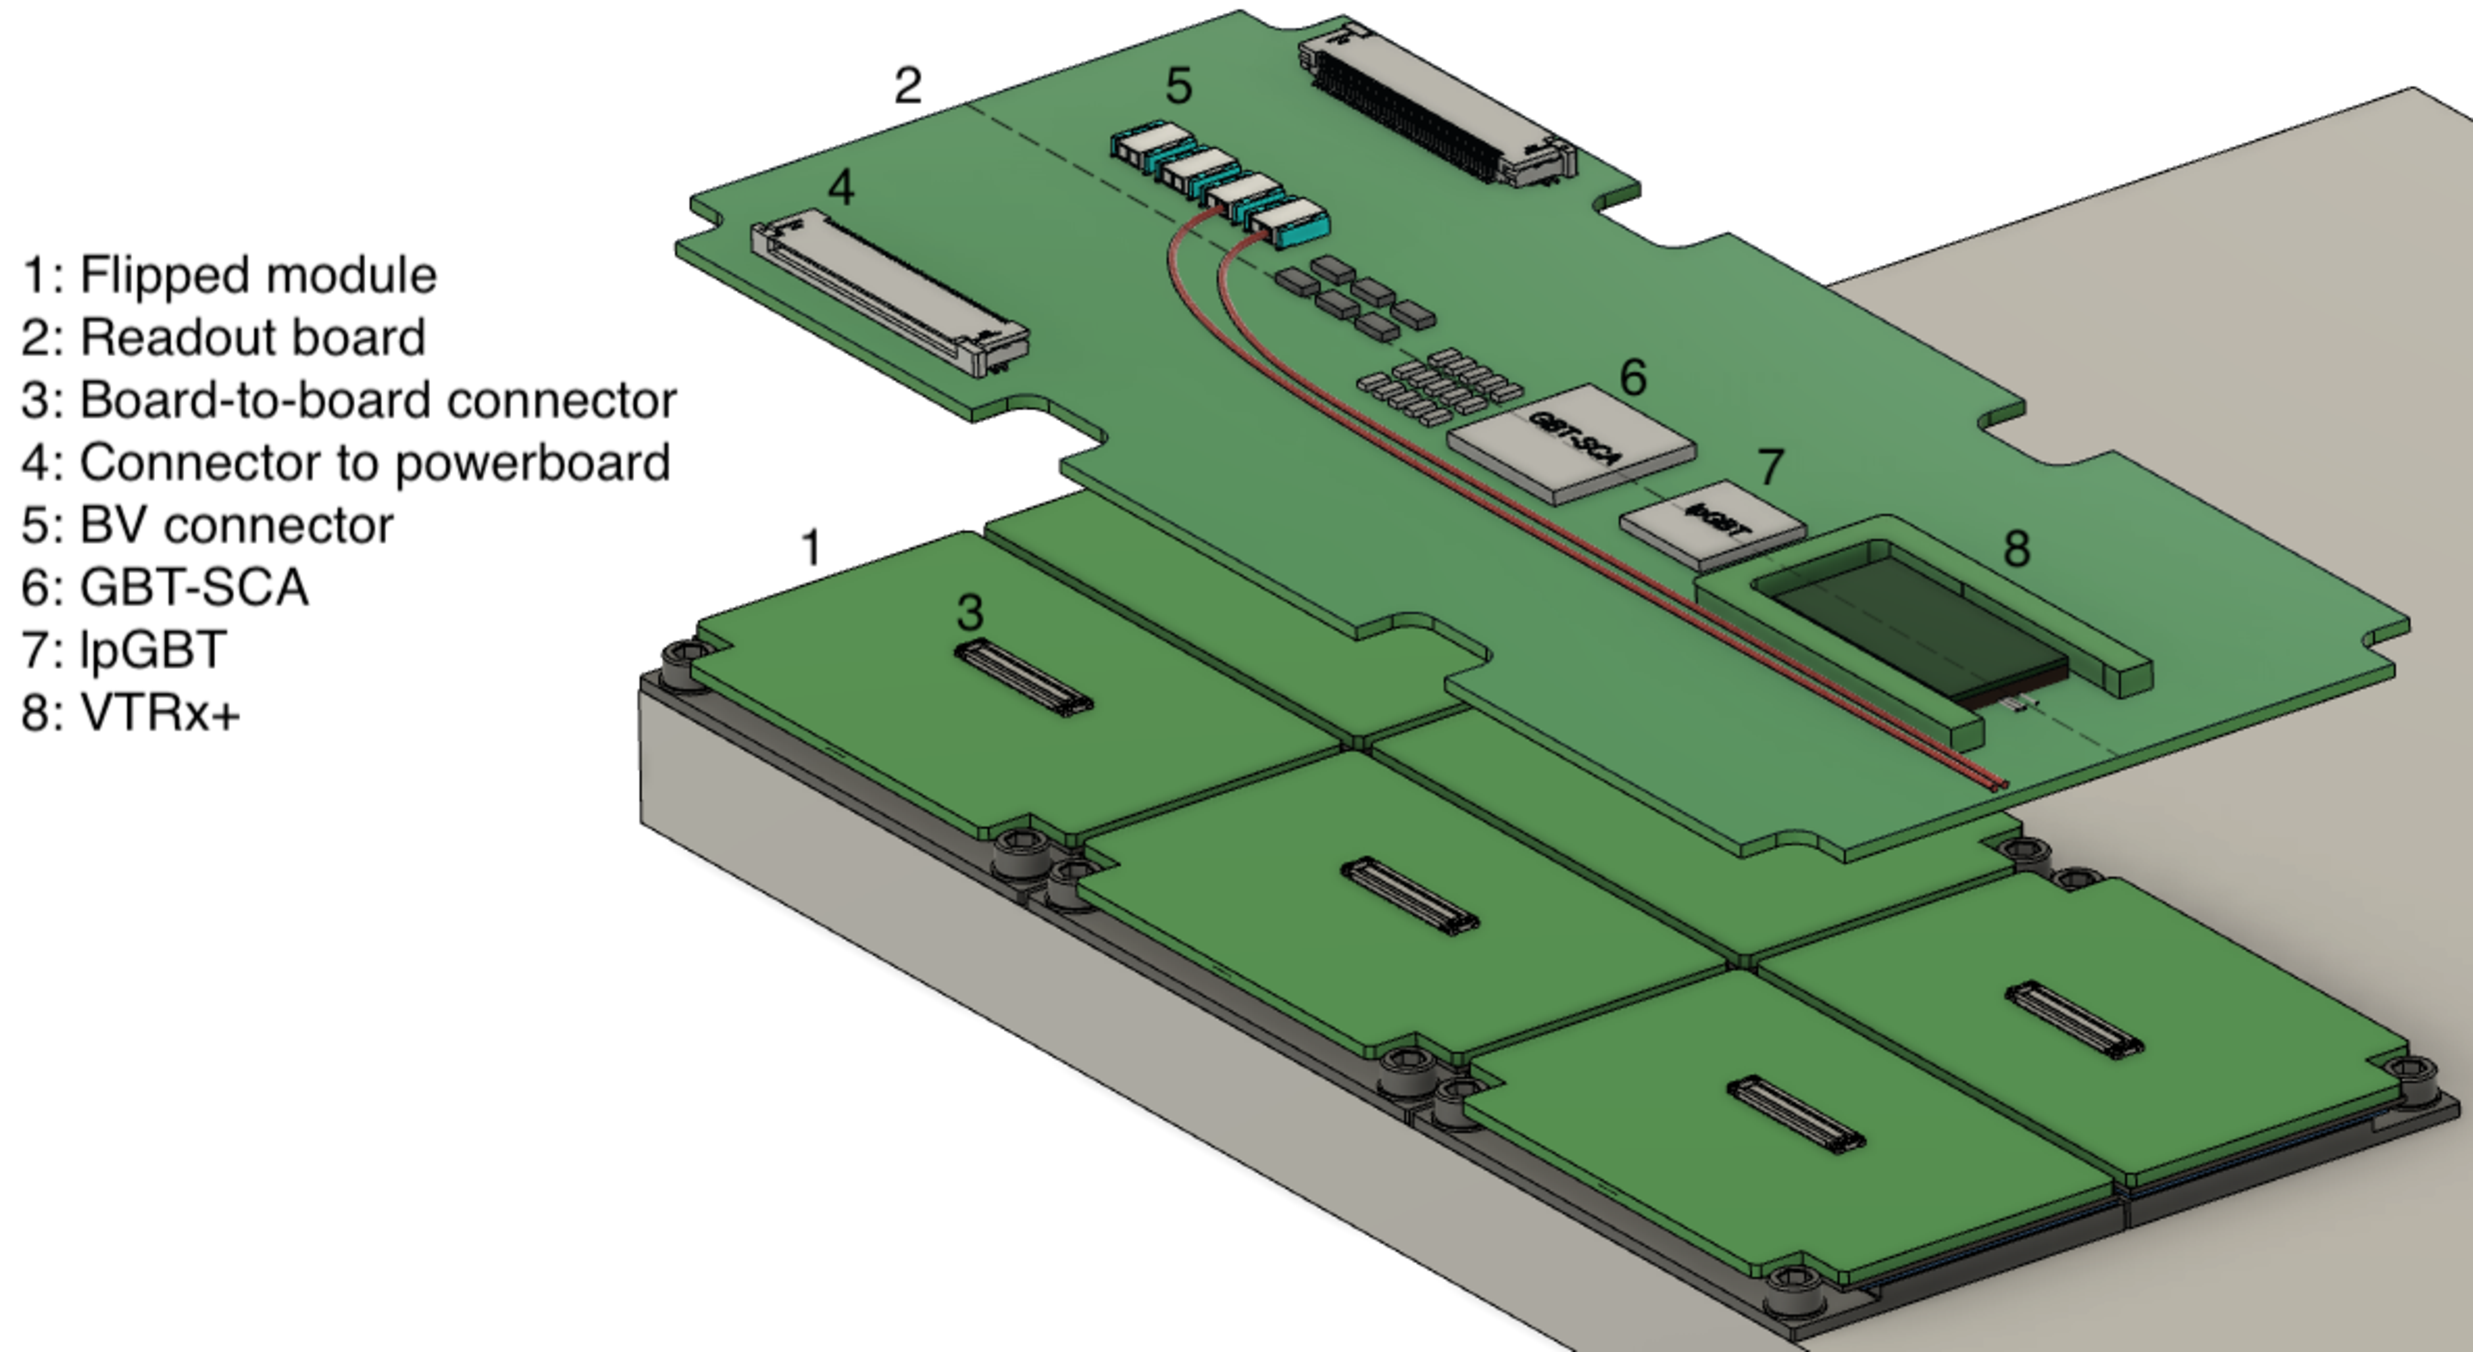
\includegraphics[width=0.90 \textwidth]{figures/ETL_exploded_legend.pdf}
  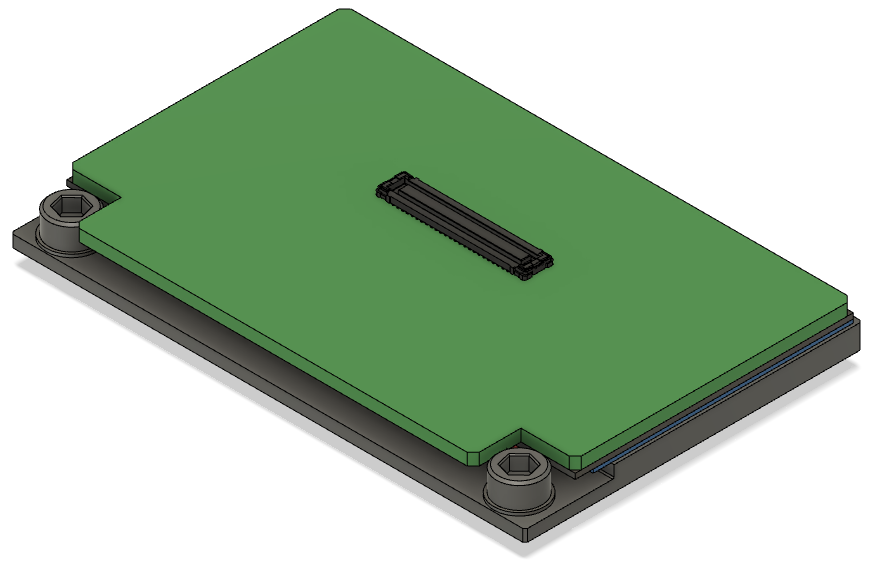
\includegraphics[width=0.40 \textwidth]{figures/Flipped_module_3D_v2.png}
  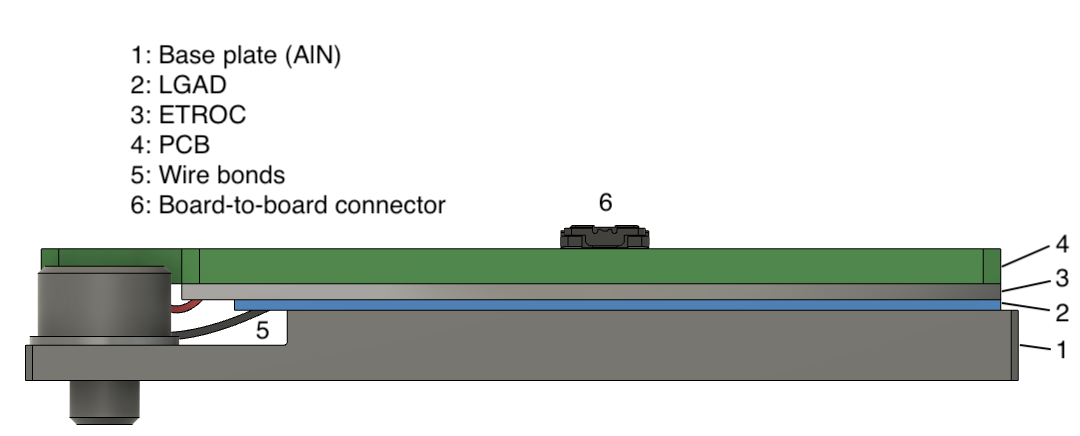
\includegraphics[width=0.55 \textwidth]{figures/Flipped_module_legend_v2.png}
  \caption{
    Top: Partially exploded views of the module-RB sandwich showing its various components.
    Bottom: View of a half module in the flipped configuration, with the LGAD sensor below the ETROC.
  }
  \label{fig:flippedModule}
\end{figure}

We foresee three different versions of the RB: covering 3 (6), 6 (12) and 7 (14) full (half) modules.
Each full module consists of two LGAD sensors and four readout chips (ETROC).

The expected radiation environment for various regions are shown in Table~\ref{tab:radiation-doses}.
To deal with higher occupancy in high-$|\eta|$ regions the innermost part of the ETL disk ($r<425~\mathrm{mm} \equiv |\eta|>2.65$) will be populated by 3-module readout boards.
The rest of the disk is organized such that the area coverage of the detector with sensors is optimized.
The layout of modules and service hybrids on the surface of the ETL wedges is presented in Figure~\ref{fig:coverage}.
Very good coverage between $1.7<|\eta|<2.8$ is achieved, without the need for half-sized modules.
We reserve an area of the width of RB and PB with a depth of 50 mm at the outer edge of the disks for MT connectors as well as LV and BV distribution, shown in Fig.~\ref{fig:patchpanel}.
The main difference w.r.t. the TDR design in terms of service hybrids is the placement of the RB on top of the modules, instead of the power board.
The RBs are powered either from above or below (powered from above shown in Fig.~\ref{fig:coverage}).

\begin{figure}[!ht]
\centering
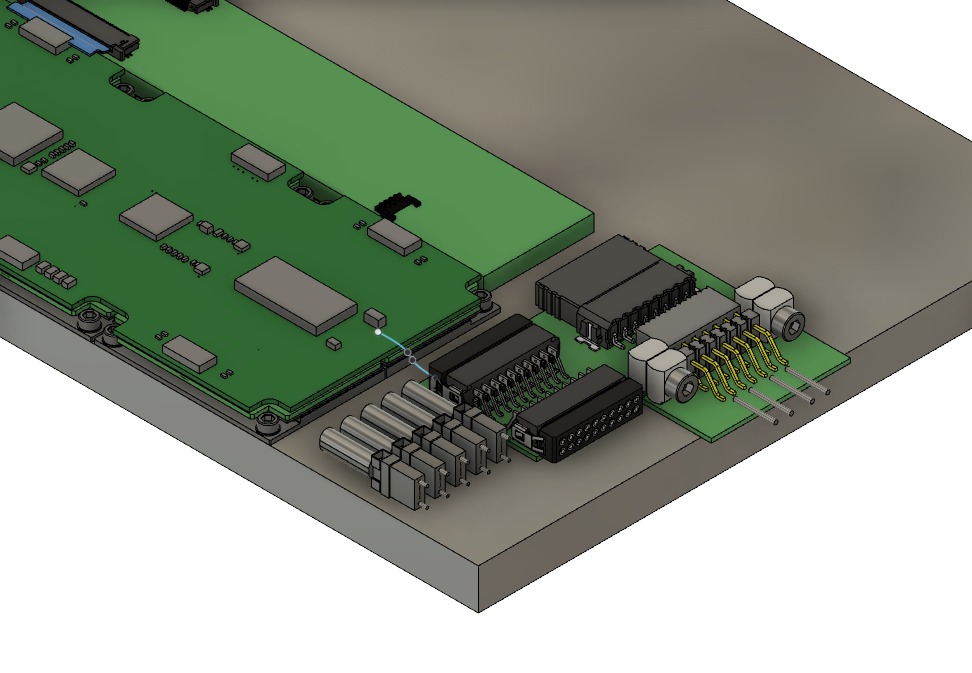
\includegraphics[width=0.70 \textwidth]{figures/patch_panel_3D.png}
\caption{
Mini-patch-panel at the end of each row of RBs and PBs.
}
\label{fig:patchpanel}
\end{figure}

\begin{table}[!hb]
  \centering
  \caption{Nominal radiation doses and fluences at various locations of the timing layers after 3000 fb$^{-1}$. The fluence is normalized to 1 MeV neutron equivalent in silicon.
  Numbers from CERN-LHCC-2019-003.}
  \begin{tabular}{ c c c c c c }
    Region & $\eta$ & R (cm) & z (cm) & Fluence (cm$^{-2}$) & Dose (kGy) \\
    \midrule
    barrel & 0.0    & 116    & 0      & 1.65$\times 10^{14}$ & 18         \\
    barrel & 1.15   & 116    & 170    & 1.80$\times 10^{14}$ & 25         \\
    barrel & 1.45   & 116    & 240    & 1.90$\times 10^{14}$ & 32         \\
    endcap & 1.6    & 127    & 303    & 1.5$\times 10^{14}$ & 19         \\
    endcap & 2.0    & 84     & 303    & 3.0$\times 10^{14}$ & 50         \\
    endcap & 2.5    & 50     & 303    & 7.5$\times 10^{14}$ & 170        \\
    endcap & 3.0    & 31.5   & 303    & 1.6$\times 10^{15}$ & 450        \\
  \end{tabular}
  \label{tab:radiation-doses}
\end{table}

\begin{figure}[!ht]
\centering
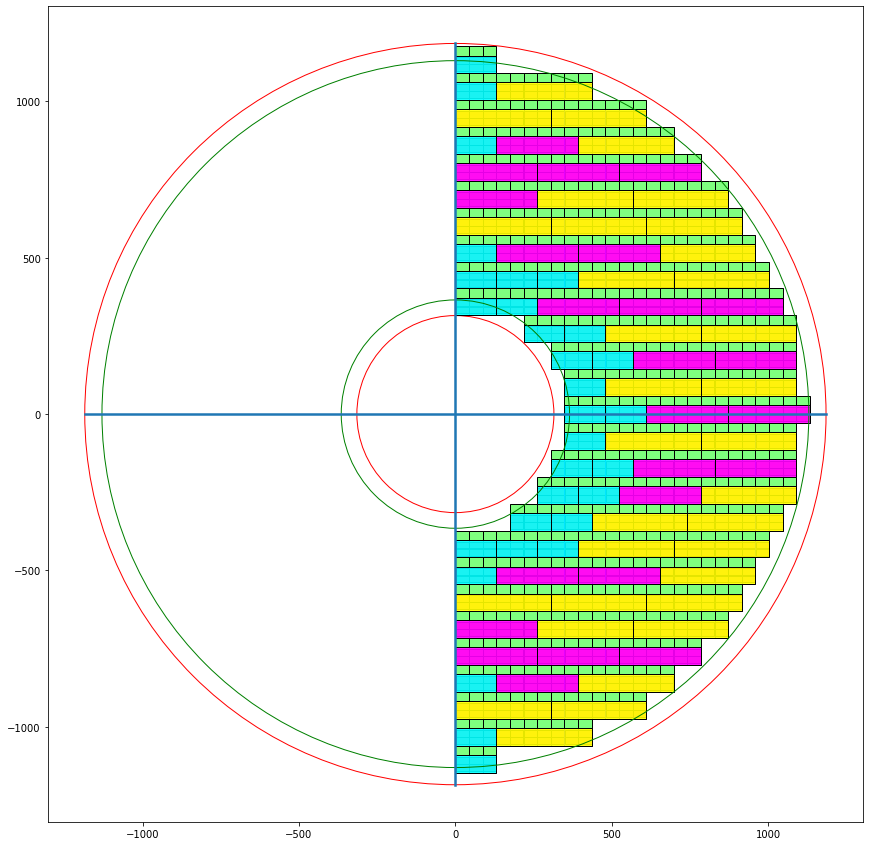
\includegraphics[width=\linewidth]{figures/coverage.png}
\caption{
Layout of various kinds of RBs on an ETL half-disk.
The red and green circles reflect the mechanical envelope of the ETL disk and the area between $1.7<|\eta|<2.8$, respectively.
Cyan, pink and yellow rectangles correspond to 3-, 6-, and 7-module readout boards.
The green rectangles indicate the reserved space above the RB for the power boards and LV services.
}
\label{fig:coverage}
\end{figure}

\begin{table}
  \caption{List of the number of each type of component used in the full ETL detector.}
  \centering
  \begin{tabular}{ l c c }
    Component type               & Number per wedge (avg) & Total number \\
    \midrule
    LGADs                        & 930             & 14,880      \\
    ETROCs                       & 1,860           & 29,760      \\
    2-sensor (full size) modules & 465             & 7,440       \\
    1-sensor (half size) modules & 0               & 0       \\
    total service hybrids     & 86.5               & 1,384       \\
    3-module service hybrids  & 28.5               & 456         \\
    6-module service hybrids  & 26.5               & 424         \\
    7-module service hybrids  & 31.5               & 504         \\
    lpGBTs, VTRX, SCA         & 86.5               & 1,384       \\
    DC-DC converters          & 915                & 14,640        \\ %9 per full-size and 5 per half-size
  \end{tabular}
  \label{tab:ETLNumberOfComponents}
\end{table}

\section{Changes to the Module Design}

In this proposal, no half size modules are foreseen.
The modules themselves have a changed structure, shown in Figure~\ref{fig:flippedModule}:
\begin{itemize}
  \item A thicker carrier (approx. 1 mm) made out of Aluminium nitride (AlN) or Aluminium oxide (alumina)
  \item The LGAD sensor is directly mounted to the carrier, below the ETROC
  \item The LGAD (BV) and ETROC (signals and LV) are wire bonded to a PCB that covers the module
  \item The module is connected to the readout board via board-to-board connectors
\end{itemize}

\section{Service Hybrid Requirements}

The proposal does not directly impact the design of the power board.
The service hybrid corridor assumed to be available for the PB is 29.5mm wide, and the full height of approximately $7.0--8.5~\mathrm{mm}$ is available for the PB, an increase in the vertical space available for the PB which may have benefits for efficiency or other aspects of the power board design.
In this proposal, the only services routed on top of the PB are the LV and DSS cables.
The connection from PB to RB is yet to be defined, but some options under consideration are:
\begin{itemize}
  \item Connection with rigid connectors, e.g. 100-mil single row right angle headers
  \item Connection with short patch cables, e.g. DF57
  \item Connection with a short flex-rigid board, with board-to-board connectors on both the powerboard and readout board.
\end{itemize}

\begin{figure}[!ht]
\centering
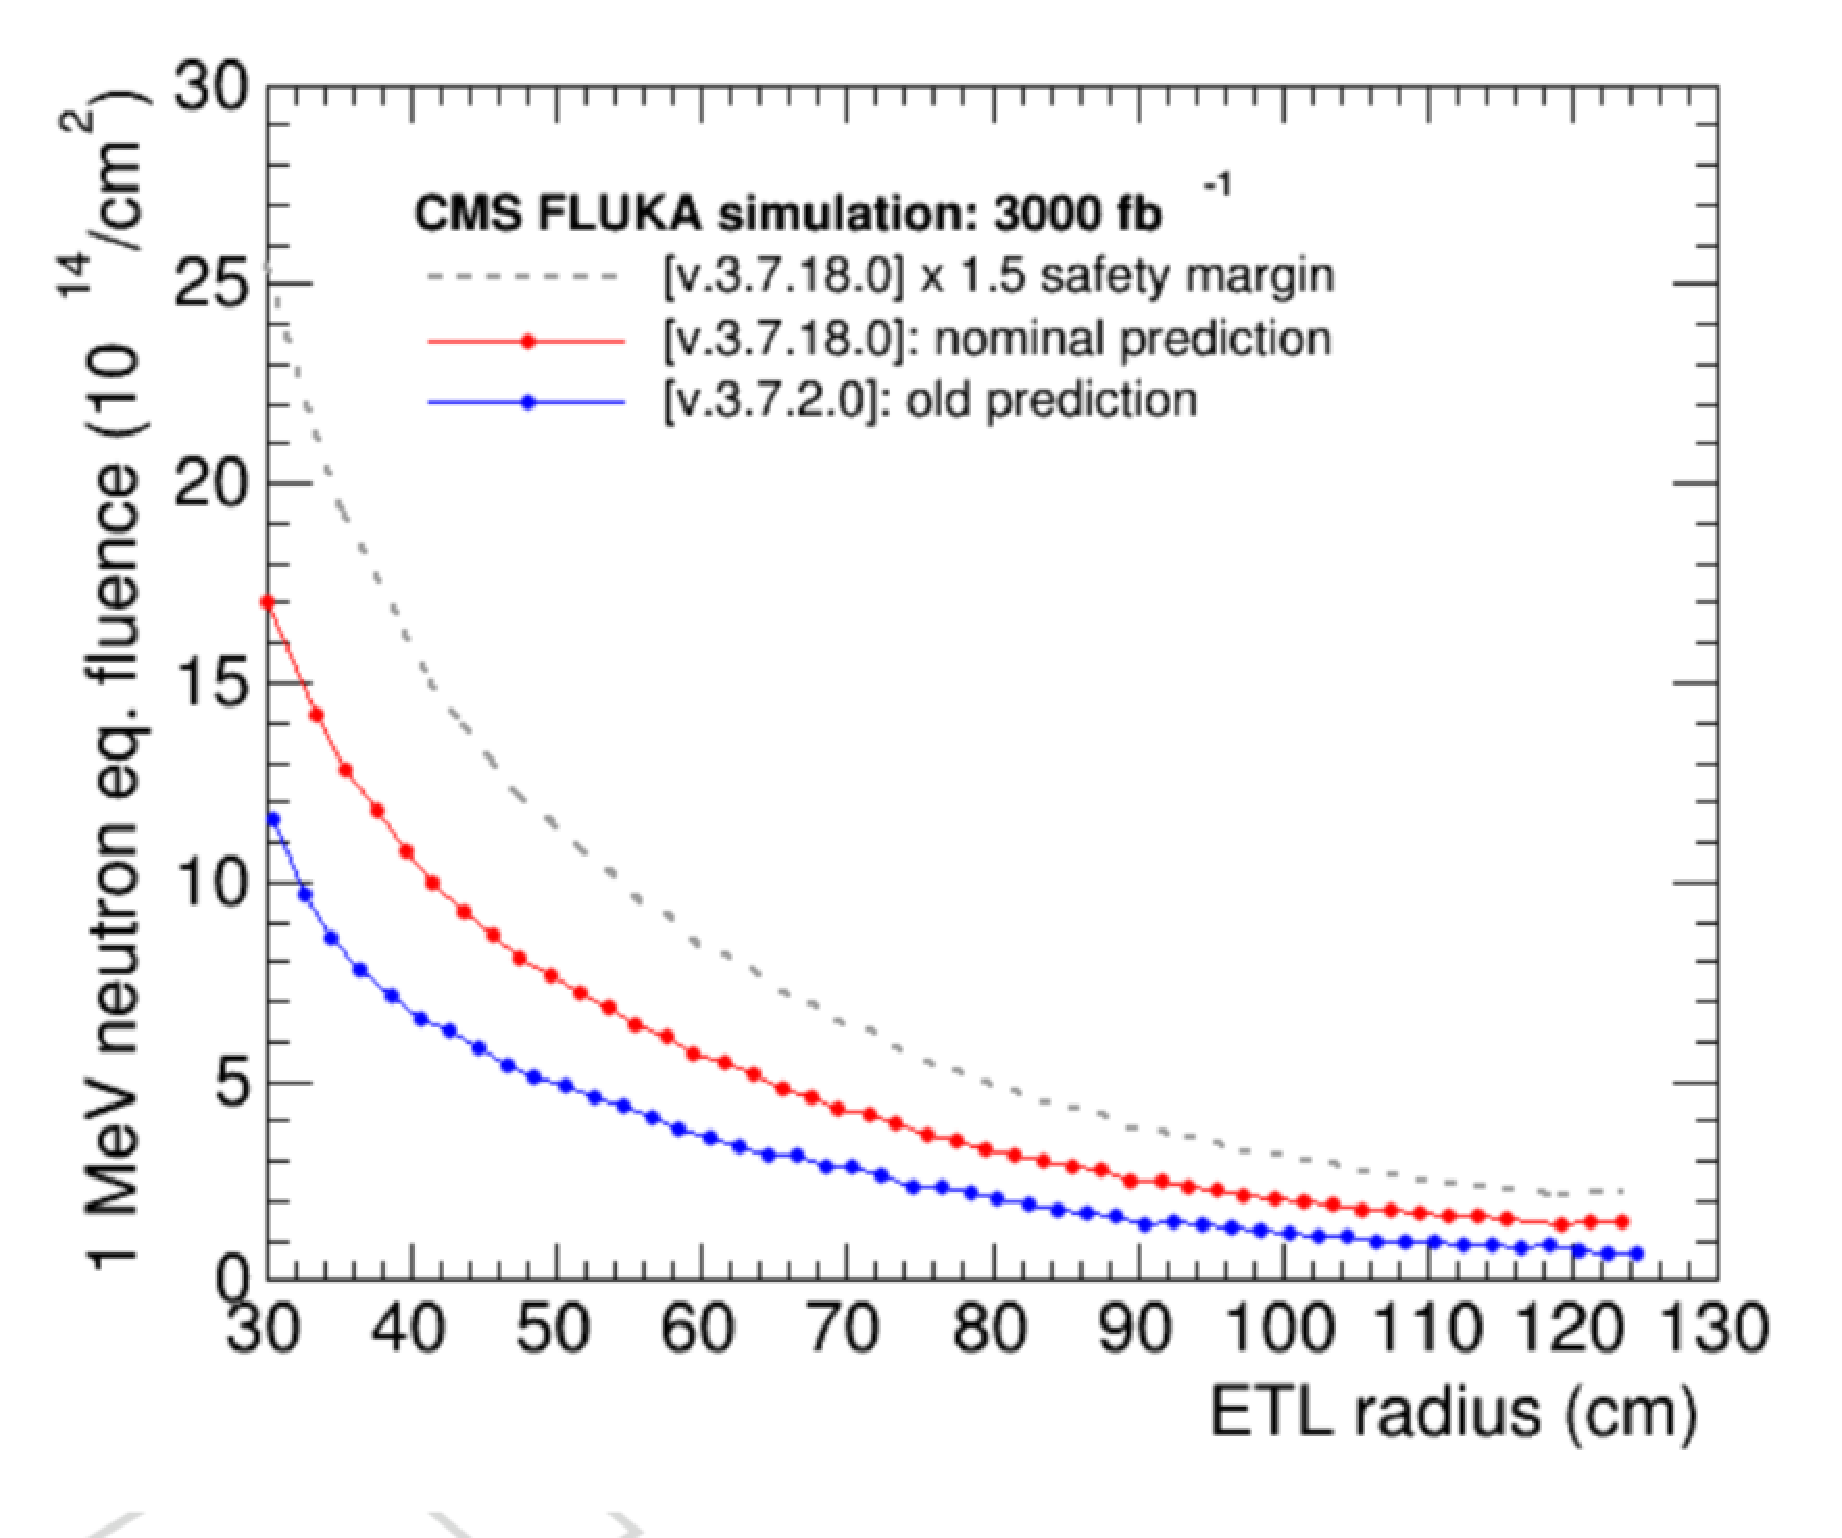
\includegraphics[width=\linewidth]{figures/image6.pdf}
\caption{
Fluence prediction in ETL for an integrated luminosity of 3000 fb$^{-1}$ from the FLUKA simulations.}
\label{fig:fluka}
\end{figure}

\section{Geometric Coverage}

We optimize the placement of modules and readout boards to achieve highest possible coverage of the ETL disk, without the need for half size modules.
The ETL disk is assumed to be limited by $r_{\mathrm{inner}}=315~\mathrm{mm}$ and $r_{\mathrm{outer}}=1185~\mathrm{mm}$, depicted by the red circles in Figure~\ref{fig:coverage_both}, corresponding to $1.659 \leq |\eta| \leq 2.950$ for an ETL position of $z=3~\mathrm{m}$.
Modules on the front and back face of each disk are arranged such that the area not covered by a sensor is minimized.
The two different arrangements are shown on the left and right of Figure~\ref{fig:coverage_both}.

In order to measure the coverage of the proposed module layout we use LGAD sensor dimensions of $22.0 \times 42.5~\mathrm{mm}$, and a full module of size $56.5 \times 43.1~\mathrm{mm}$.
A $0.5~\mathrm{mm}$ gap between each module is assumed, and the channel for the power board is taken to be $29.5~\mathrm{mm}$ wide.
Each side of the ETL detector is made of two disks (four faces) that are shifted by $2~\mathrm{mm}$ in $x$ and $y$ in order to also cover the inter-sensor gaps.

\begin{figure}[!ht]
\centering
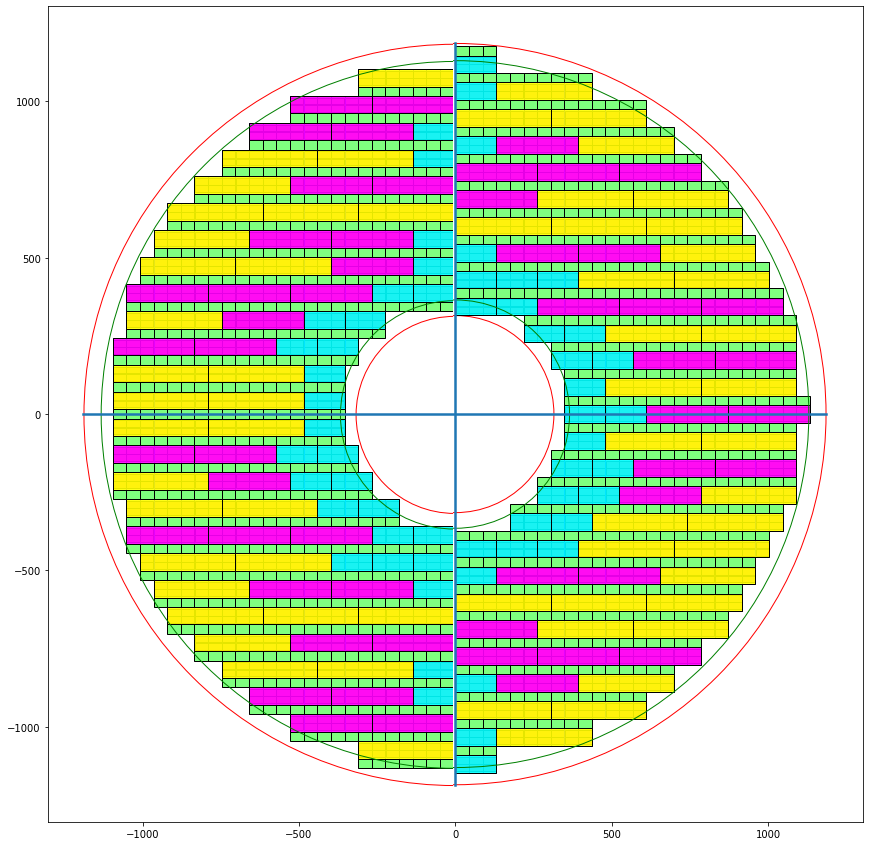
\includegraphics[width=0.60 \textwidth]{figures/coverage_both.png}
\caption{
Two half disks of the ETL detectors.
The red and green circles reflect the mechanical envelope of the ETL disk and the area between $1.7<|\eta|<2.8$, respectively.
Cyan, pink and yellow rectangles correspond to 3-, 6- and 7-module readout boards.
The green rectangles indicate the reserved space for the power boards and LV services.
}
\label{fig:coverage_both}
\end{figure}

Table~\ref{tab:coverage} shows the acceptance and geometric coverage of four different configurations of ETL modules on the disk.
The acceptance is measured by propagating muons produced at the center of CMS with $p_{T}>5~\mathrm{GeV}$ and a flat $\eta$ distribution through the CMS magnetic field to the ETL detector.
The different configurations correspond to the amount of space that is not covered by sensors at the outer edge of the disk in order to accommodate connectors (and potentially a mini-patch-panel for BV, LV and DSS).
The ``optimal'' configuration corresponds to the case where modules are placed up to the most outer edge of the disk, leaving no additional space for connectors.
In this case, 91\% of the area of the disk is covered by at least one sensor.
If 50, 65 or 85mm of space, measured along the x-axis from the modules, is kept free of modules, this geometric coverage reduces to 84--81\%.
However, due to the flat $\eta$ distribution that is used for the acceptance measurement with muons, the acceptance only reduces to 87--86\%.
For the region $1.70<|\eta|<2.80$ more than 97\% of muons intersect at least one sensor in any of the configurations.
%Approximately 96\% (70\%) of muons with $1.7<\eta<2.8$ and $p_{T}>25~\mathrm{GeV}$ produced at the center of CMS and propagated through the magnetic field have at least one (two) intersection with an ETL sensor.
An example of tracks and intersections with ETL sensors is shown in Fig.~\ref{fig:intersect}.
The majority of muons not producing any hit pass through uncovered areas at the edge of the ETL disks.
If the rapidity window is narrowed to $2.0<\eta<2.5$, more than 99\% of the muons intersect at least one of the sensors.

\begin{table}
  \caption{Acceptance for muons and geometric coverage of different configurations.}
  \label{tab:coverage}
  \begin{tabular}{c|cc|cc|cc}
    \multirow{2}{*}{Configuration} & \multicolumn{2}{c|}{$1.66<|\eta(\mu)|<2.95$} & \multicolumn{2}{c|}{$1.70<|\eta(\mu)|<2.80$} & \multicolumn{2}{c}{Geometric coverage} \\
                  & $\geq1$ hit & $\geq2$ hits  & $\geq1$ hit & $\geq2$ hits  & total & w.r.t. optimal \\ \hline
    optimal       & 0.91        & 0.79          & $>0.99$     & 0.91          & 0.91  & 1.00            \\
    50mm          & 0.87        & 0.75          & 0.99        & 0.91          & 0.84  & 0.924 \\
    65mm          & n/a         & n/a           & n/a         & n/a           & 0.83  & 0.915 \\
    85mm          & 0.86        & 0.75          & 0.97        & 0.90          & 0.81  & 0.894

  \end{tabular}
\end{table}

\begin{figure}[!ht]
\centering
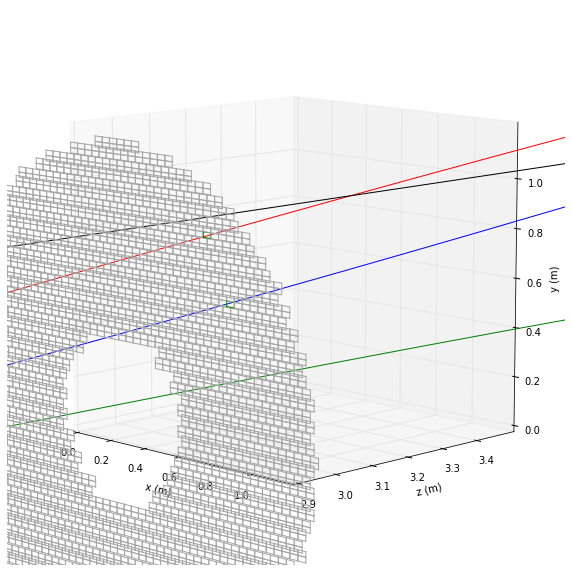
\includegraphics[width=0.70 \textwidth]{figures/intersect_3D.png}
\caption{
Tracks of three muons (red, blue, green) originating from the CMS interaction point, propagated through the CMS magnetic field.
Sensors of the first two faces of the ETL detector are shown.
Sensors that intersect the muon tracks are marked in green.
The green track passes the ETL detector without an intersection at the outer (low-$\eta$) edge of disk.
}
\label{fig:intersect}
\end{figure}

\section{Services}

At most five service hybrids are arranged in one row on the ETL disk, shown in Fig.~\ref{fig:coverage_both}.
Such a configuration is shown in Fig.~\ref{fig:services}.
LV cables can be routed on top of the PB, while the optical fibre bundles and BV cables will be routed on top of the RB.
MT connectors for the fibres are located at the end of each row, and can be accompanied by small patch panels for LV, BV and DSS connection.

\begin{figure}[!ht]
\centering
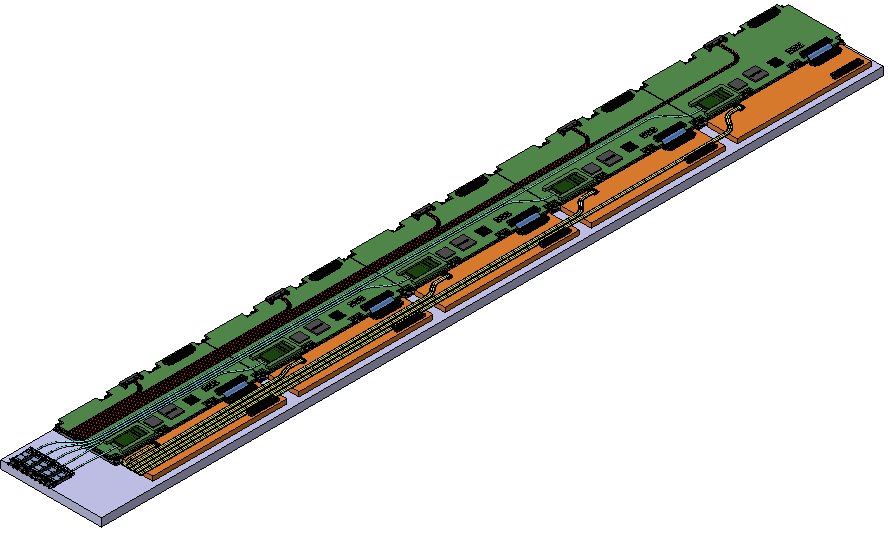
\includegraphics[width=0.90 \textwidth]{figures/services.png}
\caption{
Representation of the longest row of service hybrids, accommodating all necessary services (BV, LV, fibre bundles).
}
\label{fig:services}
\end{figure}

Moving the LV and BV connectors from the patch panel PP0 to the proposed mini patch panels at the periphery on the disk has the advantage that the connectors are easily accessible.
In the TDR concept the PP0 is located behind the two discs below the cooling lines, shown in Fig.~\ref{fig:PP0_3D}.
This makes connecting the cables to PP0 very difficult because it would be in the shadow of already installed discs.
Additionally, if no space for PP0 behind the disks is needed, the available space in z-direction for the modules/service hybrids increases from 7 mm to about 8.5 mm.
A concept of the alternative mini patch panels at the end of each row of modules and service hybrids is shown in Fig.~\ref{fig:patchpanel}.

\begin{figure}[!p]
\centering
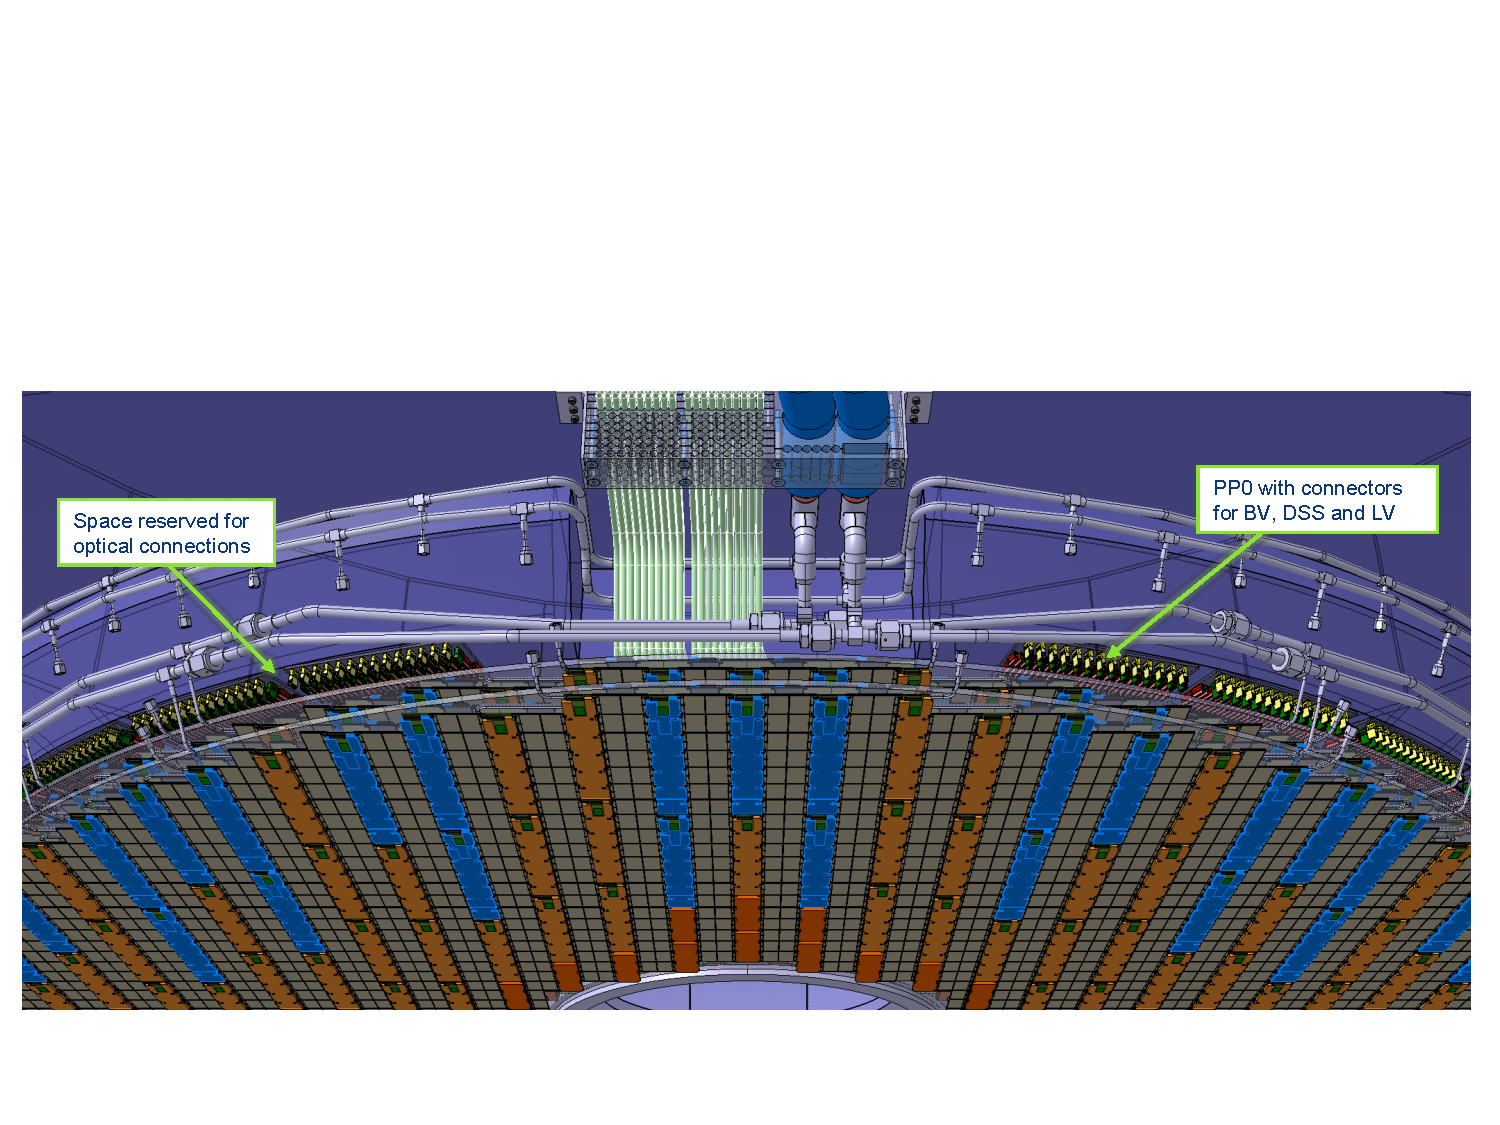
\includegraphics[width=1.00 \textwidth]{figures/PP0_3D.pdf}\\
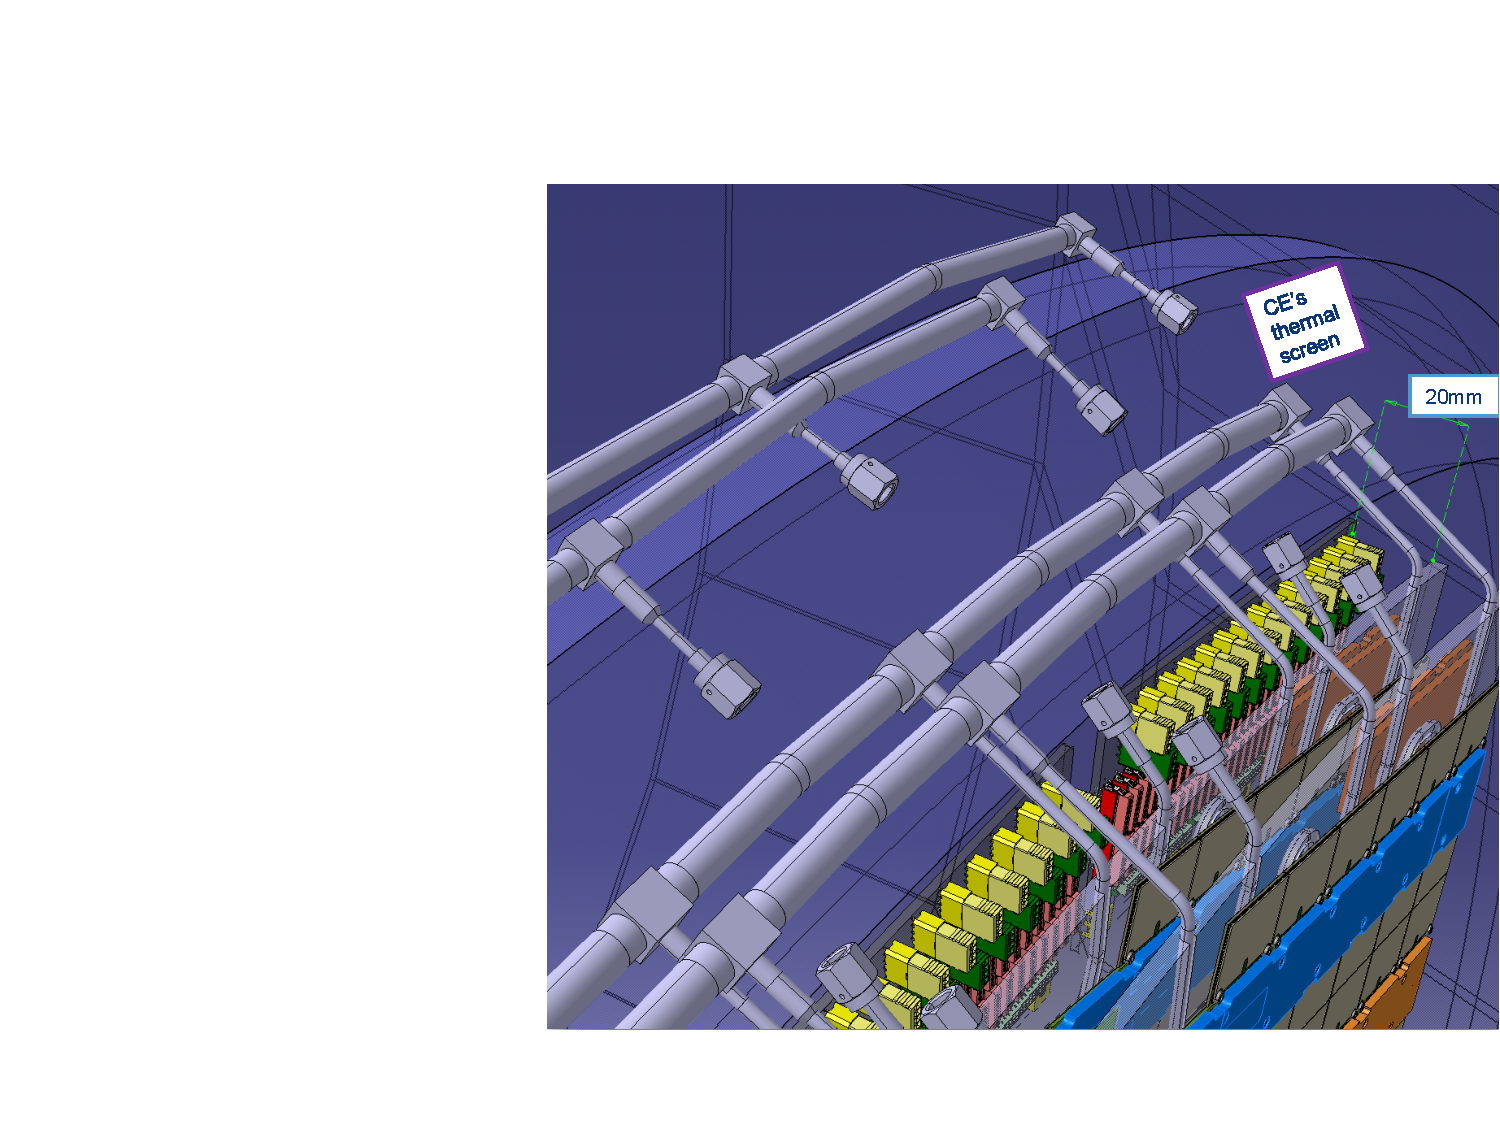
\includegraphics[width=1.00 \textwidth]{figures/PP0_location.pdf}
\caption{
Conceptual layout and location of the TDR PP0 behind the two disks.
}
\label{fig:PP0_3D}
\end{figure}

\section{Assembly and testing}

With the proposal at hand it is possible to assemble ``super-modules'' of the size of one readout board, which can then be tested and only subsequently get mounted on the ETL disk.
The assembly process would therefore be greatly simplified once the modules are assembled:
\begin{itemize}
  \item Connect modules one-by-one to the readout board
  \item If final assembly: Screw modules onto disk
  \item Connect BV cables to connectors on RB
  \item Connect RB to PB with flat cables.
\end{itemize}


\section{Potential challenges}

The following potential challenges have been identified:
\begin{itemize}
  \item The space on top of the ETL modules was reserved for service routing, which is now occupied by the readout board. Nevertheless, we have mapped out a detailed plan for the routing that fits.
  \item Thermal expansion problems of the module components: this will be tested in depth, but $\Delta T > 200C$ during bump bonding of silicon to PCBs has not caused any problems so far.
  \item Thermal conductivity: Calculations show that the temperature gradient within the silicon sensor is below 0.1K, and the temperature difference between LGAD and ETROC (across bumps) is below 1K. See Appendix \ref{sec:temperature-calculation} for details on this calculation.
  \item Thermal runaway of sensors: Should be less of a problem in this design as the sensor is directly connected to cooling.
  \item Alignment and insertion force of board-to-board connectors: We ordered connectors and will conduct studies soon.
  %\item Required space for MT connectors at the end of each row and associated loss of coverage at low $\eta$
\end{itemize}

\section{Summary}

The presented change of the ETL module and service hybrid design has several advantages over the TDR design:
\begin{itemize}
  \item Less space restrictions for RB and PB, especially vertically, giving more freedom in choice of components such as capacitors and inductors, and also allowing the power board to increase in thickness and possibly realize improvements in the embedded inductors
  \item Direct connection of RB to the module without flexi circuits, facilitating the assembly and testing processes
  \item PCB on modules allows for placement of components (e.g. bypass capacitors) close to the sensor and ETROCs
  \item No need for half sized modules
  \item Required stacking height of down to $7~\mathrm{mm}$ seems feasible
\end{itemize}

\newpage
\appendix
\appendixpage
\addappheadtotoc

\section{Temperature Gradient Calculation}
\label{sec:temperature-calculation}

One concern of the flipped module design was the possible introduction of a temperature gradient inside of the sensor, due to the changes in heat flow. In the normal design, the ETROC heat is dissipated directly through the AlN plate, while in the flipped-module design the ETROC heat must dissipate through the bump-bonds, into the sensor, and then into the AlN plate.

This introduces the possibility of temperature non-uniformity inside of the LGAD sensor. To investigate this concern, some simplified calculations were done independently by David Stuart and Frank Golf. Different assumptions about material thicknesses and conductivity were made in each calculation, but the methods are the same and the calculation was cross-checked by a third program.

The main conclusion of these calculations is that the principal concern of temperature gradients existing in the silicon, is negligible. A temperature difference of only 0.02K is predicted between the hottest and coldest parts of the sensor. This is due in large part to the relatively high thermal conductivity of silicon.

In both calculations, the common set of assumptions was:

\begin{itemize}[noitemsep,topsep=-1em]
  \item AlN Thickness = 2mm
  \item Size of a sensor pad = 1.3mm
  \item Number of bumps bonds per ETROC = 256
  \item ETROC Power = 1 Watt
  \item Bump diameter = 90 $\upmu$m
  \item Area of an LGAD = $(1.3$mm$)^{2} \times 256$ bumps $ \times 2 $ ETROCs$= 865.28$ mm$^{2}$
\end{itemize}
\vspace{1em}

The differences in assumptions between the two calculations are:

\begin{center}
  \begin{tabular}{llll}
    \textbf{Parameter}                   & \textbf{Golf}          & \textbf{Stuart}          & \textbf{Unit} \\
    \midrule
    Solder bump conductivity    & 70            & 60              & W/m$\cdot$K    \\
    Solder bump height          & 100           & 150             & $\upmu$m      \\
    Silicon sensor conductivity & 150           & 191             & W/m$\cdot$K    \\
    Silicon sensor thickness    & 300           & 200             & $\upmu$m      \\
    Epoxy conductivity          & 0.22          & 1.33            & W/m$\cdot$K    \\
    Epoxy thickness             & 500           & 1000            & $\upmu$m      \\
    AlN conductivity            & 160           & 200             & W/m$\cdot$K    \\
  \end{tabular}
\end{center}

The results of the two calculations are:

\begin{center}
  \begin{tabular}{llll}
    \textbf{Parameter}               & \textbf{Golf} & \textbf{Stuart} & \textbf{Unit} \\\midrule
    Single Bump Conductance          & 0.004         & 0.003           & W/K           \\
    Single Bump $\upDelta$t          & 0.8772        & 1.5351          & K             \\
    All bumps Conductance            & 1.140         & 0.651           & W/K           \\
    All bumps $\upDelta$t            & 0.8772        & 1.5351          & K             \\
    Sensor Conductance               & 432.640       & 826.342         & W/K           \\
    Sensor $\upDelta$t               & 0.0046        & 0.0024          & K             \\
    Epoxy Conductance                & 0.381         & 1.151           & W/K           \\
    Epoxy $\upDelta$t                & 5.2532        & 1.7379          & K             \\
    AlN Conductance                  & 69.222        & 86.528          & W/K           \\
    AlN $\upDelta$t                  & 0.0289        & 0.0231          & K             \\
    Silicon (horizontal) Conductance & 0.045         & 0.038           & W/K           \\
    Silicon (horizontal) $\upDelta$t & 0.0217        & 0.0256          & K             \\
  \end{tabular}
\end{center}

David's original notes go into detail on the methods and assumptions used in producing the calculation, and can be found at \url{http://stuart.physics.ucsb.edu/Lgbk/pub/E40756.dir/E40756.html}. His calculations are saved in a root macro which can be found at \href{http://stuart.physics.ucsb.edu/Lgbk/pub/E40756.dir/Calc.C}{Calc.C}. Backup copies of both the notes and root script are copied into the Git repository of this document at \url{https://github.com/bu-etl/readout-board-docs}

Frank's calculation can be found in a python script, accessible at: \url{https://github.com/bu-etl/readout-board-docs/blob/master/scripts/thermal_module.py}

A unified calculation used to cross-check the two can be found in a Julia script at:
\url{https://github.com/bu-etl/readout-board-docs/blob/master/scripts/thermal_module.jl}

%\clearpage
%
%\section{Bibliography}
%
%\begin{itemize}
%  \item [1]  C. Collaboration, ``A MIP Timing Detector for the CMS Phase-2 Upgrade'', CERN-LHCC-2019-003, 2019.
%  \item [2  S. Los, ``Proposal for Readout Board on Top ETL SH Stack-up'', 23 March 2020. [Online]. Available: https://indico.cern.ch/event/901444.
%  \item [3]  A. Apresyan and W. Li, ``ETL service hybrid prototyping plan'', 2020. [Online]. Available: https://cms-docdb.cern.ch/cgi-bin/DocDB/ShowDocument?docid=14040.
%  \item [4]  F. Faccio, ``The bPOL12V DCDC converter for HL-LHC trackers: towards production readiness'', in \emph{TWEPP}, Santiago de Compostela, 2019.
%  \item [5]  J. Troska, A. Brandon-Bravo, S. Detraz, A. Kraxner, L. Olanterä, C. Scarcella, C. Sigaud, C. Soos and F. Vasey, ``The VTRx+, an optical link module for data transmission at HL-LHC,'' in \emph{Topical Workshop on Electronics for Particle Physics}, Santa Cruz,, 2017.
%  \item [6]  P. Moreira, ``The lpGBT: a radiation tolerant ASIC for Data, Timing, Trigger and Control Applications in HL-LHC'', in \emph{TWEPP}, Santiago de Compostela, 2019.
%  \item [7]  A. Caratelli, S. Bonacini, K. Kloukinas, A. Marchioro, P. Moreira, R. De Oliveira and C. Paillard, ``The GBT-SCA, a radiation tolerant ASIC for detector control and monitoring applications in HEP experiments'', \emph{JINST,} vol. 10, no. 03, p. C03034, 2015.
%  \item [8]  M. O. Sahin, ``DAQ and clock -- status and schedule'', in \emph{Timing Days}, CERN, 2020.
%  \item [9]  K. DiPetrillo, ``ETROC0 Tests with FEAST Based Switching Power Supply'', ETL Meeting, 24 Nov 2019. [Online]. Available: https://indico.cern.ch/event/866436/.
%  \item [10]  S. Los, ``Power board prototyping plans'', ETL Meeting, 29 April 2019. [Online]. Available: https://indico.cern.ch/event/816963.
%  \item [11]  S. Lusin, ``ETL Integration Issues'', ETL meeting on sensors and modules, 6 Apr 2020. [Online]. Available: https://indico.cern.ch/event/906805/.
%  \item [12]  CERN, ``SAFETY INSTRUCTION IS23 -- Criteria and Standard Test Methods for the Selection of Electric Cables and Wires with Respect to Fire Safety and Radiation Resistance'', CERN, 2005. [Online]. Available:
%    https://edms.cern.ch/ui/file/335745/4/E\_IS23.pdf.
%  \item [13]  CERN, ``Safety Instruction -- The use of plastic and other Non-Metallic Materials at CERN with respect to Fire Safety and Radiation Resistance'', CERN, 2005. [Online]. Available: https://edms.cern.ch/ui/file/335806/1.02/IS41\_E.pdf.
%  \item [14]  P. Moreira, ``lpGBT -- a User's Perspective'', TWEPP, 17 Sep 2018. [Online]. Available:
%  \item [15]  J. Olsen, ``ETL DAQ and Fast Control: the view from ETROC/Front-end'', ETL meeting (Front-End Electronics), 30 Mar 2020. [Online]. Available: https://indico.cern.ch/event/902740/.
%\end{itemize}

\end{document}
